\documentclass{standalone}
\usepackage{tikz}
\usetikzlibrary{arrows.meta, positioning, shapes, fit}

\begin{document}
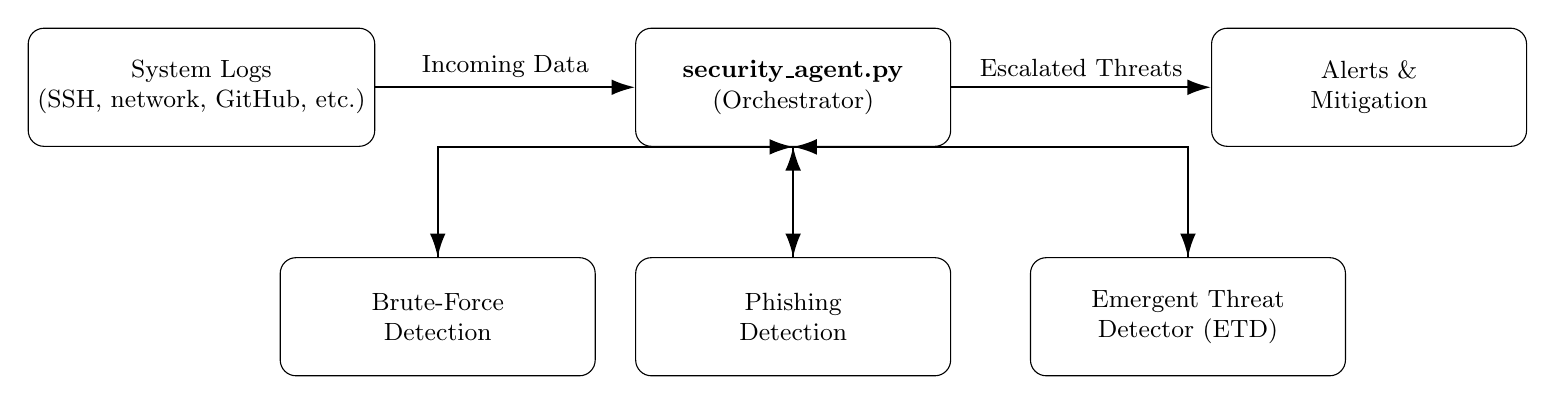
\begin{tikzpicture}[
    font=\sffamily,
    node distance=3.3cm,
    box/.style={
        rectangle, 
        draw=black, 
        fill=white, 
        rounded corners=2mm, 
        align=center, 
        minimum width=4cm, 
        minimum height=1.5cm
    },
    arrow/.style={
        -{Latex[length=3mm,width=2mm]}, 
        thick
    },
    every node/.style={font=\small}
]

% --- Nodes ---
% Row 1: Logs (left), Orchestrator (center), Alerts (right)
\node[box] (logs) {System Logs\\(SSH, network, GitHub, etc.)};
\node[box, right=of logs] (orchestrator) {\textbf{security\_agent.py}\\(Orchestrator)};
\node[box, right=of orchestrator] (alerts) {Alerts \&\\Mitigation};

% Row 2 (below orchestrator): three modules in a horizontal row
\node[box, below left=1.4cm and 0.5cm of orchestrator] (bf) {Brute-Force\\Detection};
\node[box, below=1.4cm of orchestrator] (phish) {Phishing\\Detection};
\node[box, below right=1.4cm and 1cm of orchestrator] (etd) {Emergent Threat\\Detector (ETD)};

% --- Edges ---
% Top row: logs -> orchestrator -> alerts
\draw[arrow] (logs.east) -- node[above,sloped,pos=0.5]{Incoming Data} (orchestrator.west);
\draw[arrow] (orchestrator.east) -- node[above,sloped,pos=0.5]{Escalated Threats} (alerts.west);

% Orchestrator down to modules
\draw[arrow] (orchestrator.south) -| (bf.north);
\draw[arrow] (orchestrator.south) -- (phish.north);
\draw[arrow] (orchestrator.south) -| (etd.north);

% Modules back up to orchestrator
\draw[arrow] (bf.north) |- (orchestrator.south);
\draw[arrow] (phish.north) -- (orchestrator.south);
\draw[arrow] (etd.north) |- (orchestrator.south);

\end{tikzpicture}
\end{document}